\chapter{Obecná analýza a stanovení požadavků}
V této kapitole se podíváme na možná vylepšení schopností KernelSharku. Vytvoříme pro ně požadavky a sepíšeme jejich cíle a nutné vlastnosti. Dále obecně analyzujeme, jak se dají vylepšení vytvořit. Hlubší, technická analýza každého z vylepšení pak bude součástí detailnějších pohledů na návrh a implementace vylepšení v jejich samostatných kapitolách. 

\section{Jazyk dokumenatace}
Jistě si všimneme, že tento dokument bakalářská práce je psán v češtině. Dokumentaci mimo tento dokument budeme psát anglicky. Důvodem je jž existující anglická dokumentace KernelSharku a jeho pluginů. Jelikož se jedná o open source projekt, pak je angličtina zároveň jazykem, kterému porozumí nejspíše největší množství uživatelů vylepšení.

\section{Pluginy a modifikace}
První možnou cestou rozšíření KernelSharku je přidání pluginů, které upraví zobrazované informace, nebo nějaké přidají. KernelShark již obsahuje oficiální pluginy a je možné se jejich strukturou inspirovat. Pluginy dokážou vykreslovat uživatelem definované tvary (s nimiž lze interagovat) do grafu, pozměňovat data záznamů událostí a přidávat nová menu tlačítka do hlavního okna. Pluginy tak zřejmě nejsou schopné všeho. Například nelze skrze pluginy vytvářet další záznamy, které by se pak zobrazily v grafu.

Abychom mohli docílit všech vylepšení, tak vylepšení nemohou být jen pluginy, ale i modifikace kódu KernelSharku. Přímo u zdroje je pak možné manipulovat s celým programem, nicméně na oplátku bude potřeba nerozbít to, co již funguje, zajistit podobný styl s předchozím kódem a vyznačovat místa změn, aby byla respektována licence. Obecně lze od modifikací požadovat následující:
\begin{itemize}
    \item \emph{Minimální vliv}, tj. vypnutá modifikace musí mít buď žádný, nebo minimální vliv na chod KernelSharku a jeho oficiálních pluginů. Pokud takový vliv má, musí být navržena tak, že se lze dostat ke starému chování.
    \item \emph{Stylová podobnost}, tj. kód modifikací by měl být podobný ostatnímu kódu v KernelSharku pro zachování jednotného stylu.
    \item \emph{Chovat se jako rozšíření}, tj. kód modifikací by se také měl snažit měnit existující kód co nejméně, chovat se jako rozšíření co možná nejvíce. Změny existujícího kódu musí být označeny a pokud nejsou triviální, popsány.
\end{itemize}

Od pluginů se bude obecně očekávat tento seznam:
\begin{itemize}
    \item \emph{Vlastní adresář}, tj. pluginy budou mít vždy vlastní adresář s vlastními intrukcemi pro sestavení, kódem a dokumentací, vše mimo adresář s KernelSharkem, jeho modifikacemi a oficiálními pluginy. Struktura repozitáře tímto požadavkem prospěje, pluginy budou lépe navigovatelné a kontrola nad sestavením a dokumentací pevnější. Samozřejmě je pak nutné napsat vlastní CMake instrukce k sestavení, ale to je přijatelná práce navíc.
    \item \emph{Samostatnost}, tj. pluginy by se měly snažit být co nejsamostatnější, tj. nebýt závislé na ostatních pluginech, ať už vztahem \uv{plugin A potřebuje k fungování plugin B} nebo vztahem \uv{plugin A zakazuje plugin B}. Zejména druhý ze vztahů by mohl být nepříjemný, jelikož by mohl snižovat efektivitu analýzy, některé pluginy by prostě nemohly být aktivní. První ze vztahů je mírnější, existuje hlavně pro snížení potenciálního chaosu závislostí (tzv. \uv{dependency hell}). Žádný z pluginů v této práci nebude právě z tohoto důvodu ani cílit na to být využitelný jinými pluginy jako knihovna.
\end{itemize}

\subsection{Označení modifikací v kódu}
\label{comment-style}
Licence KernelSharku, LGPL-2.1, vynucuje u provedených změn v softwaru s touto licencí jasné vyznačení změněných míst společně s datem změny. Každá změna spojena s modifikací tak bude ohraničena dvojicí komentářů:
\begin{code}
    //NOTE: Changed here. ([TAG]) ([DATE])
    ...
    // END of change
\end{code}
[TAG] je zkratkovité označení po typ modifikace, se kterou změna souvisí - každá modifikace musí mít takovou značku. [DATE] je datum napsání změny ve formátu YYYY-MM-DD. Pokud změna vznikne během vývoje nějaké modifikace, ale není na ni nutně vázána (například je to pomocná funkce s širším využitím), pak stačí ohraničit [TAG] uvozovkami.

\section{Výběr vylepšení}
Následující vylepšení umožňují v KernelSharku zobrazovat dodatečné informace, které usnadňují analýzu trasovacích událostí. Součástí jejich popisu budou i názvy těchto vylepšení, které se použijí v dalších kapitolách. Názvy budou anglické pro zachování jednotného jazyka programu. Vylepšení jsou buď pluginy nebo modifikace zdrojového kódu KernelSharku - tato informace bude také součástí jejich popisu.

Každé vylepšení, které není dodatečné, pak shrne do bodového seznamu ve vlastní kapitole hlavní myšlenky z textu své podsekce.

\subsection{Lepší analýza zásobníku kernelu}

\subsubsection*{Identifikace problémů k vyřešení}
Zaznamenávací funkcionalita KernelSharku, tzv. Record okénko, dovoluje spustit program \texttt{trace-cmd record} pro nastartování trasování běžícího systému skrze GUI. Ačkoliv to není ihned zřejmé, tato funkcionalita dovoluje uživateli dodat argumenty Trace-cmd, kterými upraví chování zaznamenávání. Pokud uživatel nezná tyto argumenty, nebude je schopen využít. Jedním z argumentů je \texttt{-T}, který zapne zaznamenávání kernel zásobníku do události typu ftrace/kernel\_stack. Zásobník je zaznamenán po každé události, kromě události zaznamenání zásobníku.

KernelShark již umí zobrazit události typu ftrace/kernel\_stack. Bere je jako každou jinou událost v trasovacích datech a tak je zobrazí jak v grafu, tak v seznamu událostí. Nicméně nás většinou nezajímá, že se nějaký zásobník trasoval, nýbrž spíš co v něm během události bylo. Z grafu toto nevyčteme, informační řádek nám nedokáže dát celou informaci, jelikož na ní nemá prostor. Seznam událostí je na tom trochu lépe, ale informace zásobníku je v textové formě víceřádková a často má řádků tolik, že většina prostoru seznamu je zabrána jen touto událostí. Celý zásobník je ovšem viditelný pouze, pokud je daná událost v seznamu vybrána, jinak se zobrazí pouze jedna řádka ze zásobníku. To nám analýzu zpomalí o vybrání zásobníkové události.

\subsubsection*{Extrakce požadavků}
Zřejmě je zde co vylepšovat. Bylo by jistě příjemnější, kdyby bylo možné zobrazit obsah zásobníku přes záznam této události v grafu, nebo vidět nějakou podstatnou část v informačním řádku, namísto klikání mezi seznamem a grafem. Toto by nemělo být realizováno přes klikání na záznam samotný, jelikož takto uživatel záznamy zvýrazňuje. V tom případě by bylo vhodnější vytvořit tlačítko nad záznamy, jejichž zásobník si chceme zobrazit. To mohou být buď přímo záznamy se zásobníkem, nebo záznamy událostí po kterých byl zásobník zaznamenán. Abychom měli záznamy kde zobrazit, bylo by nejlepší vytvořit nějaké vyskakovací okénko. V tomto okénku by mohla být vedle zásobníku i další data, například po jakém typu události byl zásobník zaznamenán, nebo jakému procesu událost patřila. Přejetím kurzoru myši přes tlačítko bychom mohli donutit informační řádek k zobrazení nějaké zajímavé části zásobníku. Abychom toho byli schopni, bude nutno KernelShark dodatečně vylepšit o akce vyvolané při přejetí kurzorem myši přes objekty v graf. Také by bylo vhodné umět toto chování nějak konfigurovat, třeba nezobrazovat tlačítka nad nějakým typem události, nebo měnit barvu tlačítek. K tomu by mohlo stačit konfigurační okénko vyvolané nějakým tlačítkem v hlavním okně. Nakonec vybereme podporované události, tj. události, pro které plugin musí fungovat. Těmi budou sched\_switch a sched\_waking. Vybrány jsou proto, že budou podstatné i u dalších vylepšení. Tím se dá testovat izolace různých vylepšení, případně i jejich kompatibilita. Zároveň jsou často zajímavé k analýze. Sched\_switch nám ukáže přepnutí z jednoho procesu na jiný. Zde lze zkoumat, proč byl proces přepnut, například zdali na něco začal čekat. Sched\_waking nám pak ukazuje změnu spícího procesu na proces připravený k běhu. Tato událost a její záznam zásobníku mlže odhalit proč lze proces opět nechat běžet, například na co se přestalo čekat.

Co se zaznamenávání zásobníku týče, ačkoliv je možné vytvořit soubor s událostmi záznamů zásobníku, bylo by uživatelsky přívětivější, kdyby se dala tato možnost zapínat pomocí nějakého GUI prvku. Nejpřirozenějším výběrem by bylo zaškrtávací políčko, umístěné v Record okénku KernelSharku. Obsah okénka nemá se zbytkem programu další vazby, tedy není třeba řešit další kompatibilitu.   

Vylepšení Record okénka je možné pouze jako modifikace, pluginy nemají k tomuto okénku přístup. Modifikaci budeme nazývat stručně jako \emph{Record Kstack}. Ovšem tlačítka nad záznamy a vyskakovací okénka je možné definovat čistě v pluginu. Jelikož bude plugin zaměřen na analýzu zásobníku, bude se nazývat \emph{Stacklook}.

\subsection{Dělení vlastnictví událostí souvisejících se dvěma procesy}

\subsubsection*{Identifikace problémů k vyřešení}
Trasování ukládá mnoho různých událostí, přičemž některé jsou svázané se dvěma procesy. Tyto procesy jsou pak touto událostí spárované. Klasickým příkladem je událost sched\_switch, tedy přepnutí se z kontextu jednoho procesu na kontext procesu jiného na stejném CPU. Trace-cmd dokáže tuto informaci uchovat, nicméně přepnutí je vyvoláno jen přepínajícím procesem. Zaznamená se tak jen jedna událost a to pro tento proces. KernelShark dokáže zobrazit ve svých CPU grafech tyto události v čase, dá se tedy zjistit, který proces byl přepnut do kterého na daném CPU. Nicméně tato informace není tak snadno zjistitelná v grafech procesů. Graf druhého procesu o přepnutí neví. Jediné, co ví, je že jeho proces začal pracovat. Pouze graf procesu přepínajícího bude o události přepnutí vědět a mít ji jako svou součást.

Tento systém, ač většinou funkční, nutí procesy se dělit o informaci, která se týká obou. Informaci pak jeden z nich ztrácí ve svém procesovém grafu. To nutí i některé pluginy upravovat vlastníky událostí, aby dosáhli svých funkcionalit. To je ovšem problém - některé pluginy mohou vyžadovat jiná data, než která jim KernelShark po upravení události dokáže poskytnout. Tedy pluginy měnící vlastníky musejí být načteny buď někdy jindy, nebo jiné pluginy zakazovat. Příkladem mohou být oficiální plugin sched\_events a další z vylepšení, \emph{Naps}. Naps plugin potřebuje mít sched\_waking události v grafu procesu, který je probouzen. Vedle toho sched\_events plugin potřebuje mít sched\_switch události v grafech procesů, na které se přepíná. Dále pak zobrazuje své tvary mezi záznamy událostí typu sched\_switch a sched\_switch, nebo mezi záznamy událostí sched\_waking a sched\_switch. Tyto dva pluginy si pak vzájemně narušují očekávaná umístění těchto dvou typů událostí a ani jeden z pluginů nefunguje správně.

Zřejmým řešením problému je pak odstranění nutnosti měnit vlastníky událostí. Například umět události rozdělit a každému z procesů dát jednu polovinu. Ale rozdělování implikuje, že by pak bylo nutné rozdělit i data z jedné události do vzniklých polovin. To ovšem není vhodné, jelikož oba procesy nejspíše budou potřebovat data celé události k efektivní analýze. Lepší bude trochu odlišný přístup. Namísto dělení události dovolíme druhému procesu z páru číst stejná data, ať už kopií události nebo odkazem na ní. Takto nerozdělíme událost samotnou, ale její vlastnictví.

\subsubsection*{Extrakce požadavků}
Podívejme se, co to znamená pro KernelShark. Záznamy událostí v KernelSharku obalují události z Trace-cmd, nebo se na ně dokážou odkázat. Jelikož KernelShark používá hlavně své záznamy, bude lepší pracovat s nimi. Z architektury KernelSharku vychází, že můžeme buď přidat umělé záznamy, které se automaticky zobrazí v grafu, nebo v grafu jenom vykreslovat objekty simulující záznam. Druhý přístup není vhodný. Simulace chování by byla zbytečně složitá na implementaci a záznamy v grafu by neodpovídaly záznamům v seznamu. Naopak první přístup jenom vytvoří umělý záznam a KernelShark se postará o zbytek. O co víc, umělé záznamy už KernelShark sám vytvářet umí během vytváření záznamů z trasovacích dat. Přístup je tedy nejen jednodušší na implementaci, ale už i používán. Vytvořené umělé záznamy by měly umět odkázat na záznam původní. Ten totiž obsahuje i původní událost a její data. Zároveň by umělé záznamy měly obsahovat data, díky kterým budou přiřazeny do správných grafů a bude možné je rozlišit od ostatních záznamů, například jménem.

S vylepšením budou muset oficiální pluginy nebo ostatní části KernelSharku umět spolupracovat. Nové záznamy by jako ostatní záznamy měly podporovat rozhraní dotazů na záznamy. KernelShark by s nimi měl také umět alespoň základně pracovat, alespoň je umět kromě zobrazení i jednoduše filtrovat. Jelikož budeme měnit chování KernelSharku, bylo by dobré umět tuto změnu chování zapínat a vypínat. Toto nastavení by mělo být uložitelné do relací. Jediný oficiální plugin, který je nutno poupravit je sched\_events.

Výše vypsané změny ukazují, že vylepšení nelze napsat jako plugin. Pouze modifikace bude schopná přidávat další záznamy do grafu a seznamu. Modifikaci nazveme \emph{Couplebreak}, podle jejího účelu rozdělit párovou událost mezi dva procesy.

Podporovanými událostmi budou sched\_switch a sched\_waking. Vybrány jsou proto, že budou podstatné i u dalších vylepšení. Tím se dá testovat izolace různých vylepšení, případně i jejich kompatibilita. Zároveň jsou to události, které pro Naps a sched\_events představují bez Couplebreaku problém a dá se na nich ukázat využitelnost vylepšení.

\subsection{Vizualizace nečinnosti procesů}

\subsubsection*{Identifikace problémů k vyřešení}
Procesy se během běhu na CPU často střídají. Důvodů může být několik - proces třeba čeká na otevření souboru, nebo mu prostě vypršel čas na CPU a byl preemptivně přepnut. Vizualizace nečinnosti v KernelSharku chybí, ačkoliv data jsou dostupná v trasovacích událostech. Pokud uživatel potřebuje zjistit předchozí stav procesu (stav před přepnutím), musí si jej najít a vyčíst v seznamu procesů. Pokud uživatel chce zjstit, jak dlouho byl proces nečinný, než byl probuzen, nezbývá mu než manuálně najít událost přepnutí a následnou událost probuzení - tato událost ovšem patří nějakému jinému procesu.

\subsubsection*{Extrakce požadavků}
Cílem vylepšení je vizualizovat pauzu mezi přepnutím procesu (sched\_switch) a probouzením jiným procesem (sched\_waking procesu, který první proces probouzí). Lze se inspirovat pluginem sched\_events, který kreslí obdélníky mezi událostmi pro něj zajímavými. Nicméně samotné obdélníky by nedokázaly nést informaci o předchozím stavu procesu, tedy nějaké barevné či textové označení bude také požadováno. Bez vylepšení Couplebreak bude nutné přesunout záznamy pro sched\_waking do grafu probouzeného procesu. S vylepšením bude stačit hledat záznamy cílových událostí probouzení. Neměli bychom se snažit kreslit obdélníky neustále. Velké množství by mohlo program zpomalovat. Mnoho záznamů na obrazovce také znamená, že budou v grafu blízko u sebe a obdělníky by pak pro sebe neměly prostor. Jelikož všechny systémy nejsou stejné, toto by mělo být konfigurovatelné v nějakém grafickém okénku. Všechny tyto změny se dají provést v pluginu.

Jelikož se bude zajímat o dobu, kdy jsou procesy nečinné, nazveme plugin \emph{Naps}, kdy naps (česky zdřímnutí) označují právě dobu nečinnosti procesu.

\subsection{Vizualizace NUMA topologie CPU vedle grafu}

\subsubsection*{Identifikace problémů k vyřešení}
KernelShark se primárně zabývá vizualizací trasovacích dat. Ovšem jenom z nich nelze vyčíst vše. Máme-li mnoho procesorů, je možné optimalizovat přístupy do paměti přes NUMA model. NUMA ve zkratce znamená, že některé procesory jsou blíže nějaké paměti či pamětem, což jejich přístupy zrychluje. NUMA tak vytváří nějakou topologii procesorů - CPU se seskupují do NUMA uzlů. NUMA uzly určují skupinu procesorů a pamětí, ke kterým mají tyto procesory blízko. Právě tu KernelShark nedokáže nijak zohlednit - procesory v grafu označuje pouze daty z trasování, pomocí indexů dodaných operačním systémem. Topologie ovšem ovlivňuje výkon aplikací s více komunikujícími procesy, nebo s procesy s pamětí na vzdáleném NUMA uzlu. Jak kernelový plánovač úloh, tak alokátor paměti se snaží NUMA lokalitu respektovat - zviditelněním  v KernelSharku bude možné analyzovat, jak dobrá tato snaha je. Program \emph{Hwloc} byl navržen právě pro zkoumání a vizualizaci topologií systémů využívajících NUMA technologii. Tento nástroj umí topologii systému i exportovat do souboru formátu XML a načíst data z takovýchto exportů. Co víc, Hwloc dokáže zachytit i zdali jsou některá CPU součástí jednoho jádra a jeví se jako samostatná CPU díky hyperthreadingu. Spojením schopností obou programů bychom mohli dodat KernelSharku možnost zobrazovat NUMA topologii procesorů systému a zároveň z grafu KernelSharku vyčíst, která část topologie byla více namáhána, než jiné.  

\subsubsection*{Extrakce požadavků}
KernelShark se zobrazováním topologií nijak nepočítá, není pro ně tedy žádná podpora. Topologie bude vytvořena pomocí programu Hwloc. Nutné tedy bude vytvořit/zabrat místo v hlavním okně, kde se bude vizualizace topologie zobrazovat. Toto místo by bylo dobré umět schovat, pokud bychom topologická data v daný moment nepotřebovali a vybrané místo by byl nevyužitý prostor. Topologii by bylo nejlepší zobrazit takovým způsobem, že CPU grafy by na zobrazení přirozeně navazovaly. Hwloc nečísluje CPU stejně jako operační systém, povolíme si tedy reorganizaci CPU grafů tak, aby byla respektována topologie. Části topologie by měly být rozlišitelné, alespoň nějakým popiskem, nebo barvou. Struktura topologie by měla být jednoduše pochopitelná, zobrazení ve stromovém stylu je zde přirozené, využívá jej Hwloc. Dále budeme muset dát uživateli nějaké okénko, ve kterém si vybere soubor s topologií, kterou chce zobrazit, a zdali topologii zobrazit chce. Soubor by vybíral pro každý otevřený stream zvlášť. KernelShark nijak nevynucuje stejný trasovaný systém v otevřených streamech, proto dává smysl toto respektovat a vybírat topologie pro každý stream odděleně. Vylepšení by také mělo být součástí ukládaných relací, už jen kvůli odstranění času stráveného hledáním a načítáním souboru topologie. Nakonec, pokud systém nevyužívá NUMA technologii, pak nemusíme zobrazovat NUMA uzly a zobrazíme pouze jádra. Ta jsou vytvořena v Hwlocu i kdyby byl hyperthreading vypnutý a jedno jádro by bylo ekvivalentní jednomu CPU.

Vylepšení bude jistě modifikací, pluginy nemají schopnosti drasticky měnit GUI. Modifikaci nazveme \emph{NUMA Topology Views}, zkratkovitě \emph{NUMA TV}.

\subsection{Dodatečná vylepšení}

Následující odstavce v rychlosti představí vylepšení KernelSharku, na která se práce nesoustředí, ovšem jejich existence KernelShark udělá trochu příjemnějším k použití a nebo jsou užitečná ve vícero jiných vylepšeních.

\subsubsection*{Aktualizace grafického kódu}
KernelShark používá Qt6 v minimální verzi 6.3.0. Nicméně Qt6 verze 6.7.0 přináší nové rozhraní pro kontrolu statusu zaškrtávacího políčka a staré rozhraní označuje při kompilaci jako zastaralé. Tato verze bude již brzy součástí hlavních Linuxových distribucí a aktualizace těchto částí kódu v KernelSharku je na místě. Dodatečným vylepšením bude modifikace kódu KernelSharku, která bude nové rozhraní využívat. Název vylepšení bude samovysvětlující \emph{Update Cbox States}.

\subsubsection*{Objekty v grafu reagují na najetí kurzoru myši}
Grafová oblast KernelSharku dovoluje uživateli dodat další tvary ke kreslení a interakci. Takové tvary jsou velmi časté u pluginů, příkladem může být sched\_events nebo Stacklook. Tyto tvary mají předdefinovaná rozhraní KernelSharkem, nicméně součástí těchto rozhraní není reakce na najetí myší přes grafický objekt. KernelShark již dokáže událost najetí myši zpracovat, využívá ji při najetí na záznamy. Jednou uživatelskou interakcí s tvary je dvojité kliknutí myši na objekt. Cílem tohoto vylepšení je dodat grafickým objektům pro grafovou oblast možnost reagovat na najetí myši a to podobným způsobem, jako je definováno dvojité kliknutí. Název tohoto vylepšení bude \emph{Mouse Hover Plot Objects}.

\subsubsection*{Využití barevných tabulek KernelSharku}
KernelShark nedovoluje využívat barvy, které používá pro procesy, CPU a streamy. Jejich využití by ale mohlo v některých případech vylepšit organizaci informací, například Stacklook může zabarvovat svá tlačítka barvou procesů, kterým události patří. Lze tak i v CPU grafu idenitifikovat vlastnící proces události, jejíž záznam zásobníku si budeme chtít zobrazit. Navíc, pokud využijeme barvy, které používá KernelShark, pak se využité barvy budou měnit společně s jinou hodnotou barveného slideru, který KernelShark uživateli zpřístupňuje. Vylepšení \emph{Get Colors} dodá KernelSharku, ve formě modifikace, dodá funkce, kterými se získají barvy momentálně využívané KernelSharkem.

\subsubsection*{Možnost měnit text v informačním řádku}
KernelShark nedovoluje měnit obsah informačního řádku. Možnost jej měnit se může hodit, pokud nějaký plugin, jako například Stacklook, by chtěl zobrazit nějaké rychlé informace uživateli. Dodatečným vylepšením bude modifikace kódu KernelSharku, která možnost měnit text v informačním řáku dodá. Vylepšení dostane název \emph{Preview Labels Changable}.

\subsubsection*{Obdélníky mezi záznamy}
KernelShark při vykreslování grafu dokresluje obdélníky mezi jednotlivé grafické reprezentace záznamů, které vyznačují aktivní proces na nějakém CPU. Tyto obdélníky jsou definovány a nakresleny během každého vykreslení na obrazovku. Ovšem ne všechny záznamy by se měly podílet na kreslení obdélníků, například záznamy zásobníku kernelu se dějí po přepnutí kontextu, kde by měl obdélník většinou skončit, a záznamy vytvořené Couplebreakem mohou chybně být začátky a konce jiných obdélníků. Vylepšení \emph{NoBoxes} jako modifikace dodá masku viditelnosti záznamů, kterou se zakáže účast na kreslení zmíněných obdélníků, a plugin, který touto maskou označí vybrané záznamy událostí.

Příklad špatného zobrazování je na obrázku \ref{obr03:modif-noboxes-bad}. Na tomto obrázku je ftrace/kernel\_stack událost vyznačená velkou svislou čarou vpravo, couplebreak/sched\_waking[target] je událost s velkou svislou čarou vlevo. Událost ftrace/kernel\_stack vytváří velký obdélník až do konce grafu, ačkoliv se událo po přepnutí kontextu a procesor ve skutečnosti po zachycení dále nepracuje. Událost couplebreak/sched\_waking[target], ačkoli neprovádí žádnou skutečnou práci na procesoru, vytváří dojem, že pracuje právě díky nakreslenému obdélníčku. V grafu CPU 1 je také velký obdélník, který začíná u události zachycení zásobníku kernelu a neměl by tedy být kreslen. Události zachycení zásobníku jsou časté a v grafu je více obdélníků spojených právě s nimi.

\begin{figure}[p]\centering
    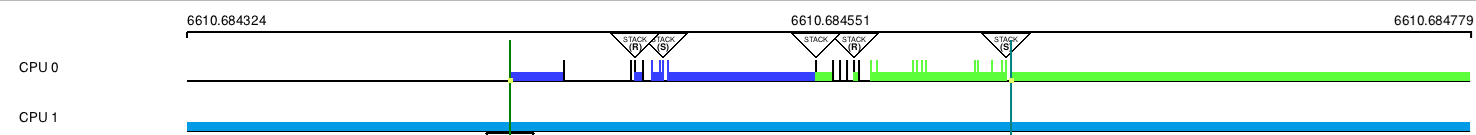
\includegraphics[width=140mm]{img/Modifikace/modif-noboxes-bad}
    \caption{Ne všechny obdélníky mezi záznamy by se měly vykreslovat, některé tvoří iluzi opravdové práce.}
    \label{obr03:modif-noboxes-bad}
\end{figure}